\scanpage{18}
\uline{Interprétations en termes de filtrations du foncteur oubli \deleted{sur la catégorie}} des représentations linéaires de dimension finie de $G$. (Il s'agit de filtrations compatibles au produit tensoriel\inserted{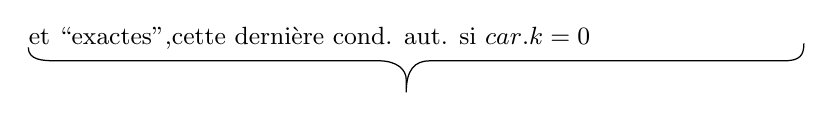
\begin{tikzpicture}[baseline=(attach)]
  \node[anchor=west,inner sep=0pt,font=\small] at (0,.35) {et ``exactes'',cette \unsure{dernière} cond. aut. si $\operatorname{car}.k=0$};
  \coordinate (attach) at (4.8,-.17);
  \draw[line width=.45pt] (0,.24) .. controls (0,.08) and (.18,.07) .. (.35,.07) -- (4.45,.07) .. controls (4.68,.07) and (4.8,-.04) .. (attach);
  \draw[line width=.45pt] (attach) -- (4.8,-.33) .. controls (4.8,-.04) and (4.91,.07) .. (5.1,.07) -- (9.6,.07) .. controls (9.8,.07) and (9.85,.14) .. (9.85,.29);
\end{tikzpicture}}). Supposons fixé une classe\inserted{\handwritten{$c$}} de\inserted{
\begin{tikzpicture}[baseline=(attach)]
  \node[anchor=west,inner sep=0pt] at (0,.27) {conjugaison, rationelle sur $k$, de};
  \coordinate (attach) at (0,-.12);
  \draw[line width=.4pt] (attach) .. controls (-.12,.18) and (.03,.13) .. (.27,.13) -- (6.1,.13) .. controls (6.3,.13) and (6.4,.23) .. (6.4,.31);
\end{tikzpicture}} telles filtrations (NB elle n'admet pas nécessairement un représentant rat/$k$); i\unsure{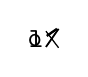
\begin{tikzpicture}[baseline=(letter.base),x=1cm,y=1cm]
  \node[inner sep=0pt,font=\ttfamily] (letter) at (0,0) {o};
  \node[inner sep=0pt,font=\ttfamily] at (.015,.015) {l};
  \draw[line width=.65pt] (.14,-.08) -- (.30,.15);
  \draw[line width=.45pt] (.14,.12) -- (.30,-.09);
  \draw[line width=.85pt] (.15,.06) -- (.28,.15);
\end{tikzpicture}} revient au même de se donner,\deleted{un} pour le Chevalley $G_o$ associé à $G$, un \deleted{homomorphisme} élément de $\operatorname{Hom}(\underline{G}_m,T_o)/W=M/W$ ($T_o=M\unsure{\mathbin{\text{\textcircled{x}}}|\otimes}\underline{G}_m$ est le tore maximal type de $G_o$) invariant par le sous-groupe\inserted{\handwritten{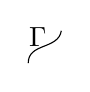
\begin{tikzpicture}[baseline=(attach)]
  \node[inner sep=0pt] at (0,.22) {$\Gamma$};
  \coordinate (attach) at (-.12,-.11);
  \draw[line width=.4pt] (attach) .. controls (-.12,.15) and (.26,.06) .. (.30,.30);
\end{tikzpicture}}} de $\operatorname{Auext}G_o=E_o$ image de $\operatorname{Gal}(\handwritten{\bar{k}}/k)$, ou encore un \deleted{homomorphisme $\underline{G}_m\unsure{\to}T$} élément de $M$ qui soit dans la chambre de Weyl de $M\mathbin{\text{\textcircled{x}}}_{\underline{Z}}\underline{R}$ et qui soit stable par $\handwritten{\unsure{\Gamma|\Gamma'}}$. On a alors le schéma $\handwritten{\underline{\varnothing}_c}$ des filtrations de classe $\handwritten{c}$, qui est un espace homogène sous $G$, de stabilisateur des points des paraboliques;\inserted{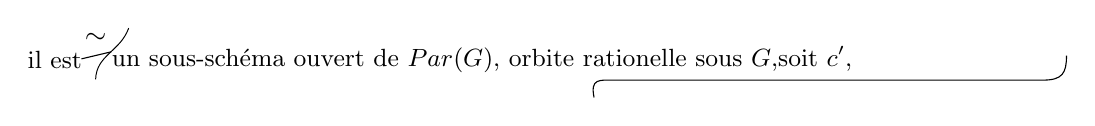
\begin{tikzpicture}[baseline=(attach)]
  \node[anchor=west,inner sep=0pt,font=\small] at (0,.38) {\handwritten{il} est};
  \node[anchor=west,inner sep=0pt,font=\small] at (1.07,.38) {un sous-schéma ouvert de $\uline{Par}(G)$, orbite rationelle sous $G$,\handwritten{soit $c'$,}};
  \node[inner sep=0pt] at (.87,.65) {\handwritten{$\sim$}};
  \draw[line width=.4pt] (.69,.39) -- (1.07,.48);
  \draw[line width=.35pt] (.87,.13) .. controls (.88,.44) and (1.18,.48) .. (1.29,.78);
  \coordinate (attach) at (7.2,-.10);
  \draw[line width=.4pt] (attach) .. controls (7.15,.14) and (7.27,.12) .. (7.43,.12) -- (12.9,.12) .. controls (13.15,.12) and (13.2,.21) .. (13.2,.43);
\end{tikzpicture}} On peut regarder aussi le schéma $\operatorname{ST}_c$ des homomorphismes $i:\underline{G}_m\handwritten{\to}G$ de classe $c$, qui est donc une orbite rationelle de $G$ opérant sur $\uline{Homgr}(\underline{G}_m,G)$. Il est canoniquement isomorphe au schéma des couples de Lévi $(P,L)$ tels que $P$ soit de classe $c'$. (En d'autres termes, grâce au choix d'un $c$, pour $P$\inserted{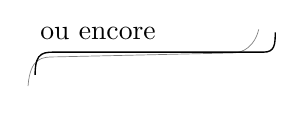
\begin{tikzpicture}[baseline=(attach)]
  \node[anchor=west,inner sep=0pt] at (0,.34) {ou encore $\handwritten{\underline{\varnothing}}$};
  \coordinate (attach) at (-.06,-.15);
  \draw[gray,line width=.25pt] (-.15,-.29) .. controls (-.12,.08) and (.03,.08) .. (.21,.08) -- (2.45,.13) .. controls (2.59,.13) and (2.73,.22) .. (2.78,.43);
  \draw[line width=.5pt] (attach) .. controls (-.06,.16) and (.05,.14) .. (.25,.14) -- (2.84,.14) .. controls (2.98,.14) and (2.99,.23) .. (2.99,.39);
\end{tikzpicture}} de classe $c'$ donné, il revient au même de se donner un $i:\underline{G}_m\handwritten{\to}P$ de la classe définie par $c$, où un sous-groupe de Lévi de $P$, à $i$ étant associé \unsure{.} $\operatorname{Cent}(i)$.\handwritten{)} On a \deleted{un homo}\inserted{deux}morphismesde schémas canoniquement isomorphes
\[
\operatorname{ST}_c\handwritten{\longrightarrow\underline{\varnothing}}_c\quad,\quad
(\operatorname{CL})_{c'}\handwritten{\longrightarrow}\operatorname{Par}_{c'}\quad,
\]
le premier en termes de théorie des filtrations \unsure{da|du} foncteurs fibres, le deuxième \deleted{d}en termes de groupes paraboliques.

Supposons maintenant que $k$ soit de car. nulle (j'ignore dans quelle mesure c'est vraiment nécessaire). On peut alors considérer le Schéma $\operatorname{Dyn}_c$ des homomorphismes $f:\operatorname{Sl}(2,k)\handwritten{\longrightarrow}G$ tels que $fi_o$ soit de classe $c$. Supposons-le non vide\inserted{\handwritten{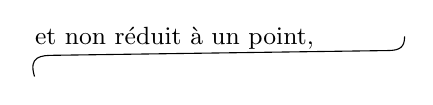
\begin{tikzpicture}[baseline=(attach)]
  \node[anchor=west,inner sep=0pt,font=\small] at (0,.34) {et non réduit à un point,};
  \coordinate (attach) at (0,-.14);
  \draw[line width=.4pt] (attach) .. controls (-.08,.12) and (.08,.13) .. (.26,.13) -- (4.48,.19) .. controls (4.64,.19) and (4.7,.23) .. (4.7,.37);
\end{tikzpicture}}}, i.e. $c$ une classe de Dynkin\inserted{\handwritten{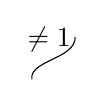
\begin{tikzpicture}[baseline=(attach)]
  \node[inner sep=0pt] at (.22,.37) {$\ne1$};
  \coordinate (attach) at (0,-.13);
  \draw[line width=.4pt] (attach) .. controls (-.04,.11) and (.56,.13) .. (.55,.41);
\end{tikzpicture}}}. Alors $\operatorname{Dyn}_c$ est un \deleted{\uline{torseur}}\inserted{\handwritten{espace homogène}} sous $G$\inserted{\handwritten{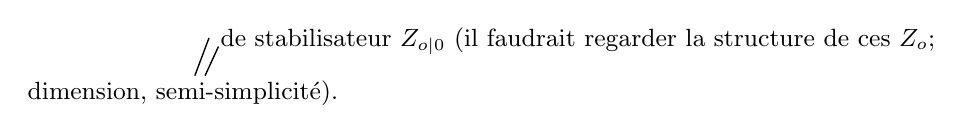
\begin{tikzpicture}[baseline=(attach)]
  \node[anchor=west,inner sep=0pt,font=\small] at (0,.42) {de stabilisateur $Z_{\unsure{o|0}}$ (il faudrait regarder la structure de ces $Z_o$;};
  \node[anchor=west,inner sep=0pt,font=\small] at (-2.45,-.24) {dimension, semi-simplicité).};
  \coordinate (attach) at (-.25,0);
  \draw[line width=.5pt] (-.32,-.02) -- (-.14,.46);
  \draw[line width=.5pt] (-.19,-.02) -- (-.02,.35);
\end{tikzpicture}}}\deleted{(en fait, il est can. is. au torseur $\uline{Isom}(G_1,G)$, où $G_1$ est le groupe quasi-déployé correspondant à $G$).} Soit $\operatorname{Un}_c$ le schéma des éléments unipotents\inserted{\handwritten{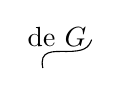
\begin{tikzpicture}[baseline=(attach)]
  \node[inner sep=0pt] at (.18,.26) {de $G$};
  \coordinate (attach) at (0,-.13);
  \draw[line width=.4pt] (attach) .. controls (-.05,.1) and (.13,.08) .. (.3,.08) .. controls (.52,.08) and (.58,.12) .. (.62,.23);
\end{tikzpicture}}} dont la classe corresponde à \deleted{celle de} $c$ par la correspondance
% archive sheet number: 17
